\chapter{On-shell techniques}	\label{onshellamp}

\section{Color decompositions in QCD}
\subsection{QCD Lagrangian and Feynman rules}
Quantum chromodynamics (QCD) is a gauge theory based on the non-abelian group $SU(N_c)$. This model describes the strong interaction between gluons and fermions. The gauge group of QCD is $SU(3)$, but we can consider a generic number of possible colors $N_c$. In addition to the utility in having an explicit dependence on $N_c$, the limit in which $N_c$ goes to infinity is sometimes useful.\\
The dynamics is described by the Lagrangian density:
$$
	\mathcal{L}_{QCD}=-\frac{1}{4} G^{a}_{\mu\nu} G^{a\mu\nu}+\sum_{f=1}^{n_f} \bar \psi_f^{i} \left(i\gamma^\mu D_\mu^{i j}-m_f \delta^{i j}\right)\psi_f^j.
$$
The first contribution is described by the gluon field tensor which can be written in terms of the gluon field $A_\mu^a$:
$$
	G_{\mu\nu}^a=\partial_\mu A_\nu^a-\partial_\nu A_\mu^a+g_s f^{abc} A_{\mu}^b A_\nu^c.
$$
The index $f$ deals with the possible flavours of quarks described by the field $\psi_f^i$ which transforms into the fundamental representation of $SU(N_c)$. Thus, in the Dirac term we used the covariant derivative in the fundamental representation:
$$
	(D_\mu)_{ij}=\delta_{ij}\partial_\mu-\frac{ig_s}{\sqrt2} T^a_{ij} A^a_{ij}.
$$
The generators $T^a_{ij}$ are Hermitian traceless $N\cross N$ matrices which carry quark indeces $i,j=1,\dots,N_c$ and a gluon index $a=1,\dots, N_c^2-1$. They obey the commutation relation
$$
	[T^a,T^b]=i\sqrt{2}f^{abc}T^c
$$
with the gauge group structure constants $f^{abc}$. The normalisation is chosen in order to avoid a proliferation of factors $\sqrt{2}$ in the sub-amplitudes. We select a diagonal basis for the generators such that
$$
	\text{tr}\left(T^a T^b\right)=\delta^{ab}.
$$
In the QCD case, explicit expressions for the $SU(N_c)$ generators can be written in terms of Gell-Mann matrices.\\
In order to extract the Feynman rules, we need to insert a gauge fixing term
$$
	\mathcal{L}_{GF}=-\frac{1}{2\xi} (\partial^\mu A_\mu^a)^2
$$
Studying the kinetic term of the Lagrangian, we can deduce the propagators for gluons and quarks.
\begin{align*}
	&\feynmandiagram [inline=(b.base), horizontal= a to b]
	{
		a [particle=\(a\mu\)] -- [gluon, momentum=\(k\)] b  [particle=\(b\nu\)],
	}; = \frac{\delta^{ab}}{k^2+i0^+}\left(\eta_{\mu\nu}+(\xi-1)\frac{k_\mu k_\nu}{k^2}\right)\\
	&\feynmandiagram [inline=(b.base), horizontal= a to b]
	{
		a [particle=\(i\)] -- [fermion, momentum=\(k\)] b  [particle=\(j\)],
	}; = \delta_{ij}\frac{\slashed k-m}{k^2-m^2+i0^+}
\end{align*}
We will specialise to the Feynman guage $\xi=1$ in which we have a simplification of the gluon propagator. 
On the other hand, the vertices are defined from the interaction terms.
\begin{align*}
	\feynmandiagram [inline=(b.base), horizontal= a to c]
	{
		a [particle=\(a\mu\)]-- [gluon, rmomentum'=\(p\)] b -- [gluon, momentum=\(q\)] c [particle=\(b\nu\)];
		b -- [gluon, momentum=\(r\)] d [particle=\(c\rho\)];
	}; = &g_s f^{abc} \left[(q-r)_\mu \eta_{\nu\rho}+(r-p)_\nu \eta_{\rho\mu}+(p-q)_\rho \eta_{\mu\nu}\right]\\[-20pt]
	\feynmandiagram [scale=0.8, inline=(b.base),horizontal= a to c, vertical= a to d]
	{
		a [particle=\(a\mu\)]-- [gluon] b -- [gluon] c [particle=\(c\rho\)],
		d [particle=\(d\sigma\)]-- [gluon] b -- [gluon] e [particle=\(b\nu\)],
	}; 
	=
	&\begin{aligned}
	&\\
	&\\[8pt]
	&-ig_s^2 \left[f^{abe}f^{cde}(\eta_{\mu\rho}\eta_{\nu\sigma}-\eta_{\mu\sigma}\eta_{\nu\rho})\right.\\
	&\left. +f^{ace}f^{dbe}(\eta_{\mu\sigma}\eta_{\rho\nu}-\eta_{\mu\nu}\eta_{\rho\sigma})\right.\\
	&\left. +f^{ade}f^{bce}(\eta_{\mu\nu}\eta_{\sigma\rho}-\eta_{\mu\rho}\eta_{\sigma\nu})\right]\\
	\end{aligned}\\
	\feynmandiagram [scale=0.87,baseline=(d.base), horizontal=d to b] {
a [particle=\(i\)]-- [fermion] b -- [fermion] c [particle=\(j\)],
b -- [gluon] d [particle=\(a\mu\)], };
= & \frac{i g_{s}}{\sqrt2} \gamma^{\mu} (T^a)_{ij}
\end{align*}
From the Fadeev-Popov approach, we know that the Lagrangian is not complete if we do not add ghosts. However, their contributions play no rule at tree-level and we will construct loop amplitudes using unitarity methods considering only physical external states which do not include ghost. 

\subsection{Counting diagrams}
In order to understand the complexity of perturbative computations when the number of legs increases, we can consider the pure gluon sector of QCD. For any diagram in the Yang-Mills theory we assign a monomial $G=g^\alpha v^\beta$, where $\alpha$ corresponds to the number of inner and external legs, while $\beta$ is the number of three-point vertices. Starting from a diagram with $n$ gluons, we can construct the contributions for the amplitude with $(n+1)$ gluon acting with differential operators on the monomials. \cite{Caravaglios_1999}
\begin{align*}
	\feynmandiagram [inline=(b.base), horizontal= a to b]
	{
		a -- [gluon] b;
	}; \mapsto
	\feynmandiagram [inline=(b.base), horizontal= a to c]
	{
		a -- [gluon] b -- [gluon] c;
		b -- [gluon] d;
	};
	\hspace{0.5cm} \boxed{\leftrightarrow} \hspace{0.5cm}
	& g \xmapsto{g^3 v \partial_g} g^3v\\
	\feynmandiagram [inline=(b.base), horizontal= a to c]
	{
		a -- [gluon,] b -- [gluon] c;
		b -- [gluon] d;
	}; \mapsto
	\feynmandiagram [scale=0.8, inline=(b.base),horizontal= a to c, vertical= a to d]
	{
		a -- [gluon] b -- [gluon] c,
		d -- [gluon] b -- [gluon] e,
	};
	\hspace{0.5cm} \boxed{\leftrightarrow} \hspace{0.5cm}
	& gv^3 \xmapsto{g \partial_v} g^4
\end{align*}
Thus we construct the monomial associated to $(n+1)$ gluons through the following differential operator:
$$
	G_{n+1}=\left(g^3 v \frac{\partial}{\partial g}+g\frac{\partial}{\partial v}\right) G_n.
$$
The number of diagrams for a tree-level amplitude with $n$ external gluons is obtained setting $g$ and $v$:
$
	N(G_n)=G_n(g=1,v=1).
$
Using this simple trick, we can count the number of diagrams for tree-level amplitudes involving only gluons in order to observe the rapid growth of complexity \cite{Badger:2016uuq}.
\begin{table}[h!]
\centering
 \begin{tabular}{||c c c c c c c c||} 
 \hline
 $N(G_3)$ & $N(G_4)$ & $N(G_5)$ & $N(G_6)$ & $N(G_7)$ & $\dots$ & $N(G_{10})$ &\\ [0.5ex] 
 \hline\hline
 $1$ & $4$ & $25$ & $220$ & $2485$ & \dots & $> 10^7$ &\\ 
 \hline
 \end{tabular}
\end{table}
\\This counting shows the necessity of reorganize the amplitudes in order to reduce the rapid combinatorial growth due to the $SU(N_c)$ color structure.

\subsection{Color factors and partial amplitudes}
Feynman rules show a structure in which we can recognise a color contribution described by the structure constants $f^{abc}$ or the matrices $T^a$ and a kinematical term. The basic idea \cite{Dixon:1996wi} consists in splitting the computation of QCD amplitudes into two parts: colour and kinematics contributions. Then we have to use a basis for colour factors: a possible choice is the reorganisation of QCD dofs in order to eliminate $f^{abc}$ in the Feynman rules in favor of the generators $T^a$.\\
With our conventions, the structure constants can be given by
\begin{align}
	f^{abc}=-\frac{i}{\sqrt{2}}\text{tr}\left([T^a,T^b]T^c \right).	\label{ftoT}
\end{align}
Pictorially, this relation can be described keeping in mind the color structure of Feynman rules.
\begin{equation*}
	 \feynmandiagram [inline=(v.base), vertical=i1 to v] 
	 { i1 -- [gluon] v -- [gluon] i2, v -- [gluon] i3,
	 };
	 =
	 \feynmandiagram [scale=0.7, baseline=-1.5cm, vertical=i1 to v1] 
	 { i1 -- [gluon] v1,
	 v2 -- [gluon] i2, 
	 v3 -- [gluon] i3,
	 v1 -- [fermion, out=180, in=120] v2 -- [fermion, out=-60, in=-120] v3 -- [fermion, out=60, in=0] v1, 
	 };
	 -
	 \feynmandiagram [scale=0.7, baseline=-1.5cm, vertical=i1 to v1] 
	 { i1 -- [gluon] v1,
	 v2 -- [gluon] i2, 
	 v3 -- [gluon] i3,
	 v1 -- [anti fermion, out=180, in=120] v2 -- [anti fermion, out=-60, in=-120] v3 -- [anti fermion, out=60, in=0] v1, 
	 };
\end{equation*}
Another important relation is the Fierz identity for $SU(N_c)$ matrices,
\begin{align}
	(T^a)_{i_1}^{j_1}(T^a)_{i_2}^{j_2}=\delta_{i_1}^{j_2}\delta_{i_2}^{j_1}-\frac{1}{N_c}\delta_{i_1}^{j_1}\delta_{i_2}^{j_2}	\label{FierzSU}
\end{align}
which corresponds to the completeness relation for the generators \cite{Henn:2014yza}. In addition, the last contribution guarantees the traceless condition.\\ %This identity is illustrated graphically with the following 't Hooft representation
%\begin{equation*}
%	 \feynmandiagram [inline=(a.base), horizontal=a to b] 
%	 { i1 -- [fermion] a -- [fermion] i2, a -- [gluon] b, 
%	 f1 -- [fermion] b -- [fermion] f2,
%	 };
%	 =
%\end{equation*}
It is sometimes convenient to consider also the $U(N_c)=SU(N_c)\cross U(1)$ gauge group. The additional generator is proportional to the identity,
$$
	(T^{a_{U(1)}})_i^j=\frac{1}{\sqrt N_c} \delta_i^j.
$$
The normalisation is chosen so that the $U(N_c)$ Fierz identity becomes
\begin{align}
	(T^c)_{i_1}^{j_2} (T^c)_{i_3}^{j_4}=\delta_{i_1}^{j_4}\delta_{i_3}^{j_2}.	\label{FierzU}
\end{align}
The $U(1)$ generator can be associated to a photon. It is colorless and presents a vanishing structure constants $f^{a_{U(1)}bc}=0$ for all $b,c$. Therefore, we do not observe any coupling between photons and gluons, while quarks carry charge under this abelian generator. In tree-level amplitudes with only gluons or at most a $q\bar q$ pair in the set of asymptotic states, the photon does not play any rule and, for this reason, we can directly simplify the computation using the identity (\ref{FierzU}) instead of (\ref{FierzSU}).\\
\subsubsection{Structure of tree gluon amplitudes}
We want to replace systematically in every Feynman diagram all the factors $f^{abc}$ in terms of the generators $T^a$. For example, we can compute the color structure of the four-gluon tree amplitude in the three channels:
$$
	c_s=f^{abe}f^{ecd}, \hspace{1cm}c_t=f^{ace}f^{edb}, \hspace{1cm}c_u=f^{ade}f^{ebc},
$$
where $a,b$ are the color indices of inner gluons and $c,d$ are associated to the out states.\\
Using equations (\ref{ftoT}, \ref{FierzU}), we can simplify the product of two structure constants,
\begin{align*}
	f^{abe}f^{ecd}&=-\frac{1}{2}\text{tr}\left( [T^a,T^b]T^e\right)\text{tr}\left([T^c,T^d]T^e\right)=-\frac{1}{2}\text{tr}\left([T^a,T^b][T^c,T^d]\right).
\end{align*}
Then we can write the four gluon amplitude as \cite{2014}
$$
	\mathcal{A}^{tree}(1,2,3,4)=g^2\left[A^{tree}(1,2,3,4)\text{tr}(T^{a_1}T^{a_2}T^{a_3}T^{a_4})+\text{perms of }(234)\right]
$$
where $A^{tree}(1,2,3,4)$ is known as a color-ordered partial amplitude.\\
We can generalise for an arbitrary number of gluons, then the colour decomposition for a gluon amplitude at tree-level is \cite{Mangano:1988kk}
\begin{align}
	\mathcal{A}^{tree}(1,2,\dots,n)=g^{n-2} \sum_{\sigma\in S_n/\mathbb{Z}_{n}} \text{tr}\left(T^{a_{\sigma_1}}\dots T^{a_{\sigma_n}}\right) A^{tree}(\sigma(1),\sigma(2),\dots,\sigma(n))	\label{trbdectree}
\end{align}
where the sum is over all the possible non-cyclic permutations of gluons.\\
Partial amplitudes show interesting relations:
\begin{enumerate}
	\item they are cyclically invariant, then we can fix the position of a gluon in the colour decomposition
	$$
		\mathcal{A}^{tree}(1,2,\dots,n)=g^{n-2} \sum_{\sigma\in S_{n-1}} \text{tr}\left(T^{a_{\sigma(1)}}\dots T^{a_{\sigma(n)}}\right) A^{tree}(1,\sigma(2),\dots,\sigma(n));
	$$
	\item they satisfy a reflection identity
	$
		A^{tree}(n,n-1,\dots,2,1)=(-)^n A^{tree}(1,2,\dots,n);
	$
	\item if we insert the $U(1)$ generator the amplitude must vanish and this yields to a linear combination known as photon decoupling identity,
	$$
		\sum_{\sigma\in \mathbb{Z}_{n-1}} A^{tree}(1,\sigma(2),\dots,\sigma(n))=0.
	$$
\end{enumerate}
The last two relations are included in a more general equation found by Kleiss and Kuijf \cite{Kleiss:1988ne}.\\
Partial amplitudes reduce the complexity, indeed we can observe a polynomial growth of necessary independent graphs for the computation of amplitudes with a different number $n$ of legs \cite{Badger:2016uuq}.
\begin{table}[H]
\centering
 \begin{tabular}{|| c | c c c c c||} 
 \hline
 $n$ & $3$ & $4$ & $5$ & $6$ & $7$ \\ [0.5ex] 
 \hline\hline
 $\mathcal{A}_n$ & $1$ &$4$ &$25$ & $220$ & $2485$ \\ 
 \hline\hline
  $A_n$ & $1$ &$3$ &$10$ & $38$ & $154$ \\ 
 \hline
 \end{tabular}
 \caption{\label{tab:FCounting}Number of needed graphs for the amplitude $\mathcal{A}_n$ and the partial one $A_n$ in function of the number $n$ of external gluons.}
\end{table}
\subsubsection{Tree amplitudes with gluons and a quark-antiquark pair}
Let us consider the scattering $q\bar{q}\rightarrow gg$. At tree-level, the amplitude is the sum of three diagrams.
\begin{align*}
\feynmandiagram [small,horizontal=a to b, inline=(a.base)] {
i1 [] -- [fermion] a -- [fermion] i2 [],
a -- [gluon] b,
f1 [] -- [gluon] b -- [gluon] f2 [],
};
\hspace{0.3cm}+\hspace{0.3cm}
\begin{aligned}
\feynmandiagram[small, vertical'=a to b]{
        i1 -- [gluon] a []
            -- [fermion] f1 [],
        a -- [anti fermion] b [],
        i2 -- [gluon ] b
            -- [anti fermion] f2
    }; 
    \end{aligned}
    \hspace{0.3cm}+\hspace{0.3cm}
     \begin{aligned}
     \begin{tikzpicture}
     \begin{feynman}
      \diagram [small, vertical=a to b] {
      i1 []
      -- [anti fermion] a
      -- [draw=none] f1 [],
      a -- [anti fermion] b,
      i2 []
      -- [fermion] b
      -- [draw=none] f2 [],
      };
      \diagram* {
          (b) -- [gluon] (f1),
          (a) -- [gluon] (f2),
      };
      \end{feynman}
      \end{tikzpicture}
      \end{aligned}
\end{align*}
For the first diagram, the colour factor can be reduced using the relation (\ref{ftoT}),
$$
	i\sqrt{2}f^{a_3a_4b}T^b=T^{a_3}T^{a_4}-T^{a_4}T^{a_3}.
$$
Thus the amplitude can be written in the following form,
$$
	\mathcal{A}^{tree}(1_{\bar q},2_q,3_g,4_g)=g^2\left(A^{tree}(1_{\bar q},2_q,3_g,4_g)T^{a_3}T^{a_4}+A(1_{\bar q},2_q,4_g,3_g)T^{a_4}T^{a_3}\right).
$$
One can demonstrate the following decomposition which generalises the expansion of the amplitude for a quark pair and an arbitrary set of gluons \cite{Mangano_1991},
$$
	\mathcal{A}^{tree}(1_{\bar q},2_q,3_g,\dots,n_g)=g^{n-2}\sum_{\sigma\in S_{n-2}}\left(T^{a_{\sigma_3}}\dots T^{a_{\sigma_n}}\right)_{i_1}^{j_2}A^{tree}(1_{\bar q},2_q,\sigma(3)_g,\dots,\sigma(n)_g).
$$
In conclusion, we can apply this reorganisation also at the loop level \cite{Bern:1990ux}. In contrast to what observed at tree level, loop amplitudes show a colour structure that does not only contain single traces. We will specify the colour decompositions in Chapter [\ref{secYM}].
\section{Spinor-helicity formalism}
In this section we will show that the kinematics of massless particle scattering in the Minkovski space $SO(1,3)$ can be described by two copies of $SU(2)$ Weyl spinors. The formalism we will review provides more compact expressions for scattering amplitudes.
\subsection{Massless particles} 
For massless particles, the projection of the spin onto the axis of the three-momentum is a conserved quantity known as helicity
$$
	h=\frac{\mathbf{p}\cdot \mathbf{S}}{|\mathbf{p}|}.
$$
We introduce the spinor-helicity language to describe efficiently on-shell scattering amplitudes. As a starting point, using Weyl basis, we can write
$$
	\slashed p =\gamma^\mu p_\mu=\begin{pmatrix}
		0 & p_{\alpha \dot\alpha } \\
		p^{\dot \alpha \alpha} & 0
	\end{pmatrix}
$$
where we introduced two objects with spinor indices. Explicitly we have
$$
	p^{\dot\alpha \alpha}=\bar \sigma^{\dot\alpha \alpha}_\mu p^\mu=
	\begin{pmatrix}
		p^{+} & \bar p_\perp \\
		p_\perp & p^{-}
	\end{pmatrix}, \hspace{0.7cm} p_{\alpha \dot\alpha}=\sigma_{\alpha \dot\alpha}^\mu p_\mu=
	\begin{pmatrix}
		-p^{-} & p_\perp \\
		\bar p_\perp & -p^{+}
	\end{pmatrix}
$$
where $\bar \sigma^{\dot\alpha \alpha}_\mu=(\mathbb{1},\sigma)$ and we introduce the light-cone coordinates $p^{\pm}=p^0\pm p^3$, $p_\perp=p^1+ip^2$.\\
In Weyl basis, Dirac equations $\slashed p u(p)=\slashed p v(p)=0$ can be converted into
\begin{align}
	p^{\dot \alpha \alpha} \lambda_{\alpha}=0, \hspace{0.5cm} p_{\alpha \dot\alpha} \tilde \lambda^{\dot \alpha}=0
	\label{Direq}
\end{align}
where $(\lambda, \tilde\lambda)$ is a pair of Weyl spinors respectively in the $(1/2,0)$ and $(0,1/2)$ representations of Lorentz group. They represent the building blocks for the solutions with defined helicity,
$$
	|p\rangle :=u_+(p)=v_-(p)=\begin{pmatrix}
		\lambda_\alpha\\
		0
	\end{pmatrix}, \hspace{0.5cm}
	|p] := u_-(p)=v_+(p)=\begin{pmatrix}
		0 \\
		\tilde \lambda^{\dot\alpha}
	\end{pmatrix}.
$$
Spinor indices can be raised and lowered with the Levi-Civita symbol $\epsilon$,
$$
	\lambda^\alpha:= \epsilon^{\alpha\beta} \lambda_\beta, \hspace{0.5cm} \tilde \lambda_{\dot\alpha}:= \epsilon_{\dot\alpha\dot\beta} \tilde\lambda^{\dot \beta},
$$
and using these objects it will be useful to define
$$
	\langle p| :=\begin{pmatrix}
		\lambda^\alpha & 0
	\end{pmatrix}, \hspace{0.5cm}
	[ p| :=\begin{pmatrix}
		\tilde\lambda_{\dot\alpha} & 0
	\end{pmatrix}.
$$
Using the properties of Pauli matrices, it is easy to show that
$$
	p_i^{\dot \alpha \alpha} p_j^{\dot \beta \beta} \epsilon_{\alpha\beta} \epsilon_{\dot \alpha \dot \beta}=2 p_i\cdot p_j.
$$
Using these property we observe that
$$
	0=p_i^2=\frac{1}{2}p_i^{\dot \alpha \alpha} p_i^{\dot \beta \beta} \epsilon_{\alpha\beta} \epsilon_{\dot \alpha \dot \beta}=\det\left(p_i^{\dot \alpha\alpha}\right),
$$
therefore we can decompose $p^{\dot\alpha \alpha}$ using only a pair $(\lambda,\tilde \lambda)$ which parametrizes a $2\cross2$ matrix with rank one. We can fix the normalisation of Weyl spinors imposing
$$
	p_i^{\dot \alpha \alpha}=\tilde \lambda_i^{\dot\alpha}\lambda_i^\alpha.
$$
Solving the equations (\ref{Direq}) with the previous condition, we obtain the explicit expressions
$$
	\lambda^\alpha=\frac{1}{\sqrt{p^+}}\begin{pmatrix}
		p^+ \\
		p_\perp
	\end{pmatrix},
	\hspace{0.5cm}
	\lambda^\alpha=\frac{1}{\sqrt{p^+}}\begin{pmatrix}
		p^+ \\
		\bar p_\perp
	\end{pmatrix}.
$$
We summarise some important identities for $SU(2)$ spinors and for their inner products.
\begin{enumerate}
	\item Angle and square brackets define the basic spinor invariants which are \textbf{antisymmetric}.
	\begin{align*}
		\langle ij\rangle&:= \lambda_i^\alpha \lambda_{j\alpha}=\epsilon_{\alpha\beta} \lambda_i^\alpha \lambda_j^\beta=-\epsilon_{\beta\alpha}\lambda_j^\beta \lambda_i^\alpha =-\langle ji \rangle\\
		[ij]&:= \tilde\lambda_{i\dot\alpha}\tilde\lambda_j^{\dot\alpha}=\epsilon_{\dot\beta\dot\alpha}\tilde\lambda_{i}^{\dot\beta}\tilde \lambda_{j}^{\dot\alpha}=-[ji]
	\end{align*}
	\item The \textbf{projection operator} is
	$$
		| i \rangle[ i |= \frac{1+\gamma_5}{2}\slashed p_i, \hspace{0.5cm} |i]\langle i|=\frac{1-\gamma_5}{2}\slashed p_i,
	$$
	and we can write 
	$
		\slashed p=|i\rangle[i|+|i]\langle i|.
	$
	We will often use the following relations in order to write traces in terms of spinor products and viceversa,
	\begin{align*}
		\langle z abc\dots xy z]=\langle z a \rangle [a b] \langle b c\rangle \dots \langle x y \rangle [y z]&= \tr \left(|a\rangle [a||b]\langle b| \dots |y \rangle[y||z]\langle z|\right)\\
		&=\tr\left(\frac{1+\gamma_5}{2}\slashed a \slashed b \dots \slashed y \slashed z\right)=:\tr_+(ab\dots yz)\\
		[z abc\dots xy z\rangle=[z a]\langle ab \rangle [bc] \dots [xy]\langle y z\rangle&=\tr\left(\frac{1-\gamma_5}{2}\slashed a \slashed b \dots \slashed y \slashed z\right)=:\tr_-(ab\dots yz).
	\end{align*}
	\item \textbf{Mandelstam invariants} can be written in terms of spinor products,
	$$
		s_{ij}:=(p_i+p_j)^2=2p_i\cdot p_j=p_i^{\alpha\dot\alpha}p_{j\alpha\dot\alpha}=\langle ij \rangle[ij].
	$$
	Viceversa we have
	$$
		\langle ij \rangle= e^{i \theta_{ij}} \sqrt{|s_{ij}|}, \hspace{0.5cm} [ij]=-e^{-i\theta_{ij}}\sqrt{|s_{ij}|}
	$$
	where $\theta_{ij}$ is a phase that can be written in terms of the components of $p_i^\mu$ and $p_j^\mu$ \cite{Henn:2014yza}.\\
	The on-shell condition $s_i:=p_i^2=0$ is manifest from the antisymmetry.
	\item Although this formalism naturally imposes the on-shell property, there are still redundancies. The condition for the \textbf{momentum conservation} imposes a relation between the spinor products,
	$$
		\sum_i p_i^\mu=0 \iff \sum_i \langle a i \rangle [ib]=0
	$$
	for arbitrary spinors $\lambda_a, \tilde\lambda_b$.\\
	We will study a formalism in which the momentum conservation will be automatically satisfied [\ref{momtw}]. 
	\item Another important relation known as \textbf{Schouten identity} comes from a basic observation of linear algebra. Any Weyl spinor can be decomposed into a basis of two others:
	\begin{align}
		\lambda_k^{\alpha}=c_i \lambda_i^\alpha+c_j \lambda_j^\alpha.	\label{Schdec}
	\end{align}
	The previous relation can be contracted with $\lambda_{i\alpha}$  or $\lambda_{j\alpha}$. Then we obtain two equations which can be solved for the variables $c_i,c_j$. Then from the relation (\ref{Schdec}) we immediately obtain the desired identity,
	\begin{align}
		|k\rangle\langle ij \rangle+|i\rangle \langle jk \rangle+|j\rangle \langle ki \rangle =0.	\label{schouten}
	\end{align}
	\item The \textbf{Gordon identity}
	\begin{align}
		\frac{1}{2}\langle i|\gamma^\mu|i]=p_i^\mu		\label{Gordon}
	\end{align}
	can be immediately shown using the property of Pauli matrices
	$$
		A=\frac{1}{2}\text{tr}\left(\sigma^\mu A\right)\bar{\sigma}_\mu,
	$$
	valid for an arbitrary complex $2\cross2$ matrix $A$.
	\item Considering an arbitrary four-vector $q^\mu$ the following contractions give the same result,
	$$
		[i|\slashed q |j \rangle=\tilde\lambda_{i\dot\alpha} q^{\dot\alpha \alpha} \lambda_{j\alpha}, \hspace{0.5cm} \langle j|\slashed q|i]=\lambda_{j}^\alpha q_{\alpha\dot\alpha} \tilde \lambda_{i}^{\dot\alpha}.
	$$
	This observation implies the \textbf{charge conjugation of currents},
	$$
		[i|\gamma^\mu|j\rangle=\langle j|\gamma^\mu|i].
	$$
	\item The \textbf{Fierz rearrangement} formula is
	\begin{align}
		\langle i |\gamma^\mu|j]\langle k|\gamma_\mu |m]=-2\langle ik \rangle[jm].
	\end{align}
	Indeed we can make explicit the sums with spinor indices and use properties of Pauli matrices,
	\begin{align*}
		\langle i |\gamma^\mu|j]\langle k|\gamma^\mu |m]&=\lambda_{i}^\alpha \sigma_{\alpha \dot \alpha}^{\mu}\tilde\lambda_{j}^{ \dot \alpha}\lambda_{k}^\beta \sigma^\nu_{\beta \dot \beta}\tilde\lambda_{m}^{ \dot \beta} \eta_{\mu\nu}=\lambda_{i}^\alpha \tilde\lambda_{j}^{ \dot \alpha}\lambda_{k}^\beta \tilde\lambda_{m}^{ \dot \beta} \sigma_{\alpha \dot \alpha}^{\mu}\eta_{\mu\nu} \sigma^\nu_{\beta \dot \beta}\\
		&=\lambda_{i}^\alpha \tilde\lambda_{j}^{ \dot \alpha}\lambda_{k}^\beta \tilde\lambda_{m}^{ \dot \beta} 2 \epsilon_{\dot\alpha\dot\beta} \epsilon_{\alpha\beta}=-2\left(\epsilon_{\alpha\beta}\lambda_{i}^\alpha\lambda_{k}^\beta\right)\left(\epsilon_{\dot\beta\dot\alpha} \tilde\lambda_{j}^{ \dot \alpha}\tilde\lambda_{m}^{ \dot \beta}\right)=-2\langle ik \rangle[jm].
	\end{align*}
\end{enumerate}
We can also describe the polarisation vectors $\epsilon_h^\mu$ for massless gauge boson with momentum $p^\mu$ and helicity $h=\pm1$ if we choose a physical gauge (the light-like axial gauge). These vectors will depend on an auxiliary light-like reference vector $n$ which arbitrariness reflects gauge invariance. The explicit solution follows from
$$
	\begin{cases}
		\epsilon_h\cdot p=0,\\
		\epsilon_h\cdot n=0,\\
		\epsilon_h\cdot \epsilon_h=0,\\
		\epsilon_h\cdot \epsilon_{-h}=-1.
	\end{cases}
$$
We can decompose the polarisation vector in an appropriate basis which contains the vectors $p^\mu, n^\mu$ and two additional directions that spans the orthogonal subspace,
$$
	\epsilon^\mu_h(p,n)=a_h p^\mu+b_h n^\mu+\frac{c_h}{2} \langle p \gamma^\mu n]+\frac{d_h}{2}\langle n\gamma^\mu p].
$$
Inserting the previous expansion in the system of equations, we obtain with the help of Fierz identities the following conditions:
$$
	\begin{cases}
		b_h=0,\\
		a_h=0,\\
		c_{h}d_{h}=0,\\
		\frac{1}{2}\langle pn\rangle[np]\left(c_{h}d_{-h}+c_{-h}d_{h}\right)=-1.
	\end{cases}
$$
An allowed solution is
\begin{align}
	\epsilon_+^{\mu}(p,n)=-\frac{\langle n\gamma^\mu p]}{\sqrt{2}\langle np \rangle},\hspace{0.5cm}\epsilon_-^{\mu}(p,n)=\frac{\langle p\gamma^\mu n]}{\sqrt2 [pn]}.	\label{solepsilon}
\end{align}
\iffalse
\subsection{Massive case}
We will focus on the use of spinor helicity formalism for massless particles, but we can generalize this language to treat the properties of massive particles. For massive particles helicity is not a Lorentz-invariant object, but it is only defined with respect to the direction $n^\mu$ which breaks Lorentz-invariance. A possible approach is to find directly the eigenvectors of the momentum matrix $p_{\alpha\dot\alpha}$ to obtain the solutions for the massive Dirac equation. Alternatively, we can decompose the time-like momentum $p_i$ into two light-like directions: a null reference $q_i$ and the vector $$(p_i^b)^\mu=p-\frac{n^2}{2p\cdot n} n^\mu.$$
If $m\not=0$ the determinant of the momentum matrix does not vanish, therefore it has the maximum rank. Then we have to use two pairs of Weyl spinors to describe completely $p_{\alpha\dot\alpha}$. Precisely, we can use the following decomposition:
\begin{align*}
	p_i^{\dot\alpha \alpha}&=\bar \sigma_{\mu}^{\dot\alpha\alpha}p^\mu=\bar \sigma_{\mu}^{\dot\alpha\alpha}\left((p^b_i)^\mu+\frac{m^2}{2 n\cdot p}n^\mu\right)\\
	&=(\bar\sigma\cdot p^b_i)^{\dot\alpha\alpha}+\frac{m^2}{2p\cdot n}(\bar\sigma\cdot n)^{\dot\alpha\alpha}\\
	&=\tilde \lambda_{p^b_i}^{\dot\alpha}\lambda_{p^b_i}^{\alpha}+\frac{m^2}{2p\cdot n}\tilde \lambda_{n}^{\dot\alpha}\lambda_{n}^{\alpha}=:\tilde\lambda_{iI}^{\dot\alpha} \lambda_i^{\alpha I}.
\end{align*}
We can use an additional index $I=1,2$ to write the sum over a spinor basis which is defined by a double copy of spinor pairs. Details about the spinor-helicity formalism for all masses and spins can be found in \cite{Arkani-Hamed:2017jhn}.
\fi
\section{Momentum twistors} \label{momtw}
The spinor-helicity solves the on-shell constraints but we still have some redundancies. First of all, spinors must satisfy the momentum conservation:
\begin{align}
	\sum_i \lambda_i^a \tilde \lambda_i^{\dot a}=0.	\label{momcons}
\end{align}
In addition, starting from $6$ points, we observe other constraints in four dimension, indeed only four vectors are independent. For example in the case of six particle, we need to satisfy the Gram determinant condition,
$$
	\text{Gram}(p_1,p_2,p_3, p_4, p_5)=0,
$$
which gives a complicated polynomial relation.\\
The constraints reduce the number of independent variables to $3n-10$ for an amplitude with $n$ particles. This is exactly the number of dofs for an amplitude invariant under Poincarr\'e transformations with on-shell legs. Then all the conditions we have to impose are on-shellness, momentum conservation and Gram determinants. We want to construct a system of variables in which all the constraints are trivially satisfied.\\

The momenta $p_i^\mu$ can be used to construct graphically a figure with a closed contour due to the momentum conservation. We can use the colour ordering to select a specific polygon. We can decide to describe the kinematics using coordinates from the dual-space:
\begin{align*}
	&y_i^{\dot aa}-y_{i+1}^{\dot a a}=p_i^{\dot a a},\\
	&y_i^{\dot aa}-y_j^{\dot aa}=p_i^{\dot aa}+p_{i+1}^{\dot aa}+\dots + p_{j-1}^{\dot aa}.
\end{align*}
While the momenta $p_i$ are the sides, the variables $y_i$ correspond to vertices of the polygon. Dual coordinates make the momentum conservation manifest,
$$
	p_1+p_2+\dots+p_n=(y_1-y_2)+(y_2-y_3)+\dots+(y_n-y_1)=0.
$$
Using these coordinates and Dirac equation for massless particles, we can observe the so-called incident relation:
\begin{align}
	\lambda_i^{\alpha}(y_i)_{\alpha\dot\alpha}=\lambda_i^{\alpha}(y_{i+1})_{\alpha\dot\alpha}=:(\mu_i)_{\dot\alpha}.
	\label{incidentrel}
\end{align}
This define a new variable $\mu_i$ that we can use to describe the kinematics of the scattering process. More precisely, we can consider the set $Z_{iA}=(\lambda_{i\alpha},\mu_i^{\dot\alpha})$ as an alternative parametrisation compared with the use of four-momenta or spinor-helicity components $(\lambda_i,\tilde\lambda_i)$. $Z_i$ are called momentum twistors and their geometrical structure is described for example in \cite{2014}.\\
Any line based on the dual-space and defined by the points $y_i$ and $y_{i+1}$ corresponds to a point $Z_i$ in the twistor space. Viceversa, $y_i$ can be determined knowing $Z_i$ and $Z_{i+1}$, then for any line in the twistor space we observe a point in the manifold parametrised by the dual coordinates. Indeed we can show that
$$
	(y_{i})_{\alpha\dot\alpha}=\frac{\lambda_{i\alpha}\mu_{i-1,\dot\alpha}-\lambda_{i-1,\alpha}\mu_{i,\dot\alpha}}{\langle i-1|i \rangle}.
$$
Momentum twistors solve automatically the three types of constraints: on-shell conditions, momentum conservation and Gram determinants.\\
%We can describe the spinor $\tilde \lambda_i$ in terms of momentum twistor variables. The starting point is
%\begin{align*}
%	&\langle i | i-1 \rangle \langle i+1 | p_i= \langle i| i-1 \rangle \langle i+1 |(y_{i+1}-y_i)\\
%	&\langle i | i-1 \rangle \langle i+1 | i \rangle [i|=\langle i| i-1 \rangle \langle i+1 |y_{i+1}-\langle i| i-1 \rangle \langle i+1 |y_i
%\end{align*}
%and we can apply Schouten identity in the last addend,
%\begin{align*}
%	&\langle i | i-1 \rangle \langle i+1 | i \rangle [i|=\langle i| i-1 \rangle \langle i+1 |y_{i+1}+\langle i+1|i\rangle\langle i-1|y_i+\langle i-1|i+1\rangle \langle i| y_i\\
%	&\langle i-1 | i \rangle \langle i | i+1 \rangle [i|=\langle i | i-1 \rangle[\mu_{i+1}|+\langle i+1|i\rangle[\mu_{i-1}|+\langle i-1|i+1\rangle[\mu_i|\\
%	&\tilde\lambda_i=\frac{\langle i+1|i\rangle\mu_{i-1}+\langle i-1|i+1\rangle\mu_i+\langle i | i-1 \rangle\mu_{i+1}}{\langle i-1 | i \rangle \langle i | i+1 \rangle}.	\numthis \label{tildelambda}
%\end{align*}
In order to obtain a map between the spinor-helicity formalism and momentum twistors, we can write $\tilde \lambda_i$ in terms of $Z$. Using the incident relation (\ref{incidentrel}) and Schouten identity (\ref{schouten}), we can prove the relation
$$
	\tilde\lambda_i=\frac{\langle i+1|i\rangle\mu_{i-1}+\langle i-1|i+1\rangle\mu_i+\langle i | i-1 \rangle\mu_{i+1}}{\langle i-1 | i \rangle \langle i | i+1 \rangle}.
$$
Using the previous relation, we can directly prove the constraint (\ref{momcons}).
%In a compact form, the spinors $\tilde\lambda_i$ can be extracted from the dual twinstor,
%$$
%	W_i^A=(\tilde \mu_{i\alpha},\tilde \lambda^{\dot\alpha}_i)=\frac{\epsilon^{ABCD}Z_{i-1,B}Z_{i,C}Z_{i+1,D}}{\langle i-1|i\rangle\langle i|i+1\rangle}
%$$
Amplitudes can be parametrized using the holomorphic spinor products and momentum twistor 4-brackets:
\begin{align*}
	\langle ijkm \rangle= \epsilon^{ABCD}Z_{iA}Z_{jB}Z_{kC}Z_{mD}.
\end{align*}
In conclusion, a $n$-point massless amplitude can be described by $n$ momentum twistors. Any $4\cross n$ matrix for $Z$ will generate $n$ momenta such that all the constraints in four dimension are trivial. This matrix is parametrised by $(3n-10)$ variables $x_i$, but the choice is not unique. We used the following invertible parametrisation for the matrix.
\begin{align}
	Z=\begin{pmatrix}
		1 & 0 & \frac{1}{x_1} & \frac{1}{x_1}+\frac{1}{x_1x_2} & \frac{1}{x_1}+\frac{1}{x_1x_2}+\frac{1}{x_1x_2x_3}&  \dots&\frac{1}{x_1}+\dots+\frac{1}{x_1x_2\dots x_{n-3}} &\frac{1}{x_1}+\dots+\frac{1}{x_1x_2\dots x_{n-2}} \\
		0 & 1 & 1 & 1 & 1 &\dots& 1 &1\\
		0 & 0 & \frac{x_{n-1}}{x_{2}} & x_{n} & x_{n+1}& \dots  & x_{2n-6} & 1\\
		0 & 0 & 1 & 1 & x_{2n-5} & \dots  & x_{3n-11} & 1-\frac{x_{3n-10}}{x_{n-1}}
	\end{pmatrix}
	\label{momparamet}
\end{align}
A practical advantage of this choice is that the Gram determinant of four momenta becomes a perfect square in the momentum twistor variables. For example, if we consider a five-point amplitude, using (\ref{momparamet}) we have
\begin{align*}
	\text{Gram}(p_1,p_2,p_3, p_4)&=\left[\frac{x_1\left(x_2(1+2 x_3)x_4-(1+x_3)x_4(x_4-x_5)+x_2^2x_3(-1+x_5)\right)}{x_2}\right]^2\\
	&\equiv\left[\text{tr}(\gamma_5 \slashed p_1 \slashed p_2 \slashed p_3 \slashed p_4)\right]^2=: (\text{tr}_5)^2.
\end{align*}
The momentum twistor variables $\{x_1,\dots,x_5\}$ are equivalent to the set $\{s_{12},s_{23},s_{34},s_{45},s_{51},\tr_5\}$. Using the choice (\ref{momparamet}) we have rational maps which connect the two system of variables which describe the kinematical dependence of the amplitude for five massless particles.
\subsection{One off-shell leg}
The principal aim of this project is to study an amplitude involving four massless particles and a massive field. For this reason, we want to extend the formalism of momentum twistors for an amplitude with one off-shell external leg.\\
We can consider the massive leg with momentum $p_5$ as an off-shell particle which decays into two massless states.
\begin{center}
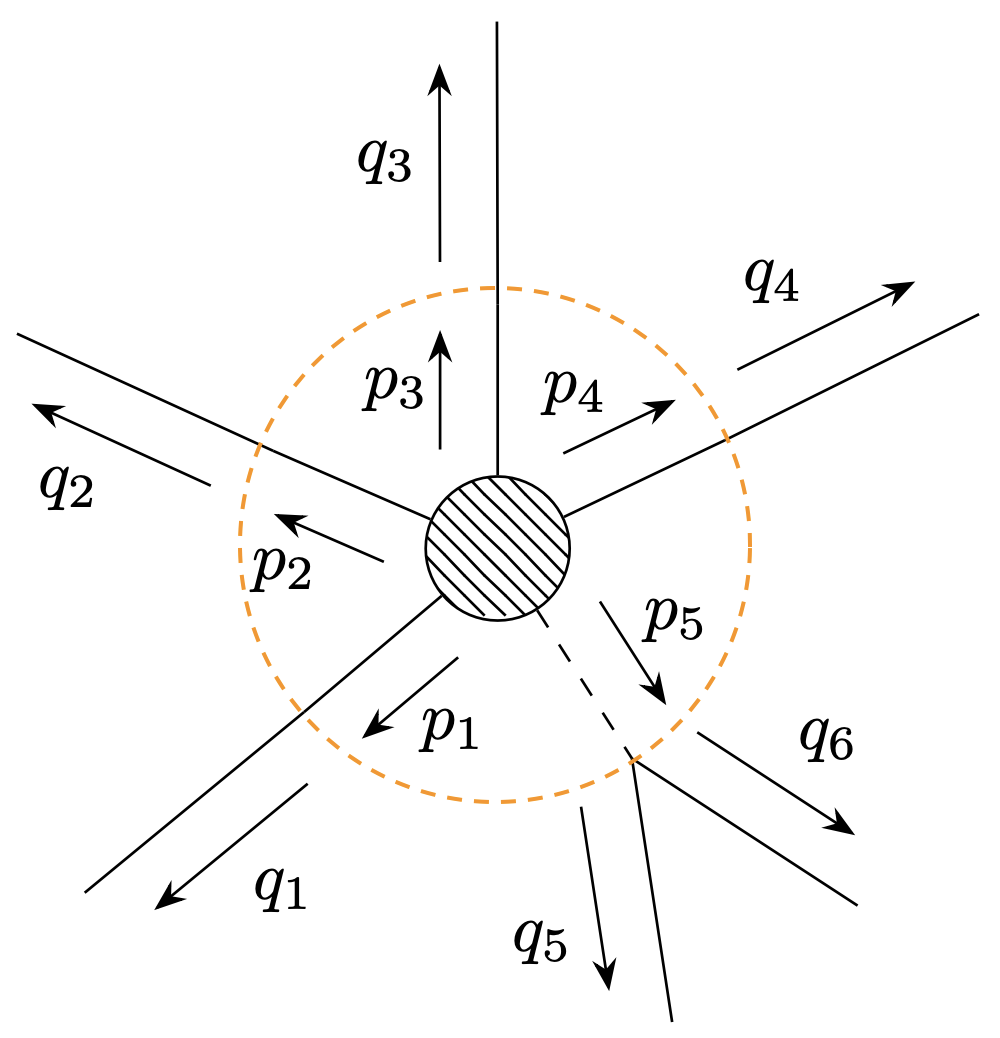
\includegraphics[width=0.40\textwidth]{massiveZ}
\end{center}
We can generate $q^\mu$ using momentum twistors for a $6$-point massless amplitude. The idea is to reconstruct $p_5^\mu$ in terms of twistor variables using the condition $p_5=q_5+q_6$.\\
Before doing it,  we need to carefully organise the degrees of freedom. Indeed an amplitude with six asymptotic massless states requires $3\cdot 6-10=8$ independent variables. On the other hand, an amplitude with five particles and one mass parameter presents $3\cdot5-10+1=6$ variables. In order to match the number of dofs, we can impose additional constraints. For example, we required that the complex momentum $q_6$ is collinear to $q_2$, i.e.
$$
	[q_2q_6]=0\hspace{0.35cm}\text{and}\hspace{0.35cm}\langle q_2q_6\rangle=0.
$$
We obtain a parametrisation for the momentum twistors. In terms of the new variables, we can express the standard kinematical variables which describe a five-point amplitude with an external mass,
\begin{align*}
	&s_{12}=x_1,\\
	&s_{23}=x_{1}x_4,\\
	&s_{34}=x_1\left(\frac{(1+x_3)x_4}{x_2}-x_3(1+x_4(-1+x_5))\right),\\
	&s_{45}=x_1x_6,\\
	&s_{51}=x_1x_3(x_2-x_4x_5),\\
	&s_{5}\equiv(p_5)^2=\frac{x_1x_3(x_2-x_4)\left(x_4(x_5-1)+x_6\right)}{x_4},\\
	&\text{tr}_5=\frac{x_1^2}{x_2}\left[x_2^2x_3(1+x_4(x_5-1))+(x_3+1)x_4(x_4-x_6)+x_2(x_4(x_3(x_5-3)-1)+x_3x_6)\right],
\end{align*}
and inversely we can express $x_i$ in terms of $\{s_{ij},s_{5},\text{tr}_5\}$ as explicitly described in \cite{Badger:2021ega}.\\
In conclusion, the five-point amplitude with a massive particle $5$ will be decompose as follows,
$$
	A(1,2,3,4,5)=h \cdot f(s_{ij},s_{5},\text{tr}_5),
$$
where $h$ is the helicity factor which encodes the phase information of the amplitude. If we use momentum twistors during a computation, we have to isolate the factor $h$ before the last passage in which we change the variables from $\{x_i\}$ to $\{s_{ij},s_{5},\text{tr}_5\}$ in order to avoid losing information.
\section{Tree-level recursion relations}
Tree-level amplitudes can be computed in principle summing all the possible diagrams constructed with Feynman rules. Unfortunately, we already observed that the complexity significantly increases with the number of asymptotic states. Nevertheless it, the result is often much simpler than the intermediate steps. For example, in the case of two negative gluons and an arbitrary number of bosons with a negative helicity, QCD amplitudes are encoded by the Parke-Taylor formula \cite{Parke:1986gb},
\begin{align}
	A^{tree}(1^+,\dots, (i-1)^+,i^-,(i+1)^+,\dots(j-1)^+,j^-,(j+1)^+,\dots, n^+)=\frac{\langle ij \rangle^4}{\langle 12 \rangle \langle 23 \rangle\dots \langle n-1|n\rangle\langle n1 \rangle},	\label{PT}
\end{align}
although the number of diagrams which contribute increases with the legs.\\
In this section, we discuss techniques to overcome the complexity of computations with Feynman graphs. Firstly, we will review an approach based on a off-shell current to construct gluon amplitudes. In the second part of the section, we will review recursion relations which use on-shell amplitudes as building blocks. %For this reason, these on-shell relations overcome the complexity due to the gauge redundancy of Feynman diagrams.
\subsection{Off-shell recursion relations}
We introduce the off-shell current $J^\mu$ which represents the sum of colour-ordered $(n+1)$-point Feynman graphs with a single off-shell leg $\mu$ and $n$ on-shell states. The amplitude will be
$$
	A_{n+1}=J^\mu(1,2,\dots,n) \epsilon_\mu(n+1).
$$
$J^\mu$ is called Berends-Giele current and it satisfies conditions which come from the property of the amplitude. It is conserved, i.e. $J\cdot (p_1+\dots p_n)=0$, and it satisfies the reflection and the photon decoupling identities,
\begin{align*}
		&J^\mu(n,n-1,\dots,2,1)=(-)^{n+1} J^\mu(1,2,\dots,n),\\
		&J^\mu(1,2,3,\dots,n)+J^\mu(2,1,3,\dots,n)+\dots + J^\mu(2,3,\dots,n,1)=0.
\end{align*}
We can construct $J^\mu$ recursively attaching the off-shell leg with other gluons using three-point and four-point vertices and contracting those legs with similar currents with fewer legs. We can describe pictorially the relation with the following picture \cite{Berends:1987me}.
\begin{align*}
	J^\mu(1,\dots,n)
	&=\sum_{k=1}^{n-1} \begin{aligned}
	\feynmandiagram [small, layered layout, horizontal=a to b] {
	a [particle=\(\mu\)] -- [gluon] b [blob] -- [gluon] f1 [blob, label={15:\hspace{0.1cm}\(\bullet\)}], b -- [gluon] c [blob, label={-15:\hspace{0.1cm}\(\bullet\)}],
	f1 -- [gluon] f11 [particle=\(1\)],
	f1 -- [gluon] f12 [particle=\(k\)],
	c -- [gluon] c1 [particle=\(k+1\)],
	c -- [gluon] c2 [particle=\(n\)], 
	}	;
	\end{aligned}
	+\sum_{k=1}^{n-2} \sum_{l=k+1}^{n-1}
	\begin{aligned}
	\feynmandiagram [small, layered layout, horizontal=a to b] {
	a [particle=\(\mu\)] -- [gluon] b [blob] -- [gluon] f1 [blob, label={15:\hspace{0.1cm}\(\bullet\)}], b -- [gluon] d [blob, label={-15:\hspace{0.1cm}\(\bullet\)}], b -- [gluon] c [blob, label={0:\hspace{0.1cm}\(\bullet\)}],
	f1 -- [gluon] f11 [particle=\(1\)],
	f1 -- [gluon] f12 [particle=\(k\)],
	c -- [gluon] c1 [particle=\(k+1\)],
	c -- [gluon] c2 [particle=\(l\)],
	d -- [gluon] d1 [particle=\(l+1\)],
	d -- [gluon] d2 [particle=\(n\)] 
	}	;
	\end{aligned}
\end{align*}
The starting point of the recursion is $J^\mu(i^{\pm})=\epsilon^\mu_{\pm}(p_i, q_i)$.\\The first non-trivial current is 
$$
	J^\mu(1,2)=\begin{aligned}
	\feynmandiagram [small, layered layout, horizontal=a to b] {
	a [particle=\(\mu\)] -- [gluon] b [blob] -- [gluon] f1 [blob], b -- [gluon] c [blob],
	f1 -- [gluon] f11 [particle=\(1\)],
	c -- [gluon] c2 [particle=\(2\)], 
	}	;
	\end{aligned}=J(1)\cdot J(2) (p_1-p_2)^\mu+2 J^\mu(2) p_2 \cdot J(1)-2 J^\mu(1) p_1\cdot J(2).
$$
Using Berends-Giele recursion relations, we can check that
$$
	A_n(1^+,2^+,\dots,(n-1)^+,n^\pm)=0
$$
for increasingly numbers of gluons. Changing the polarisation, we can also verify (\ref{PT}) for some values of $n$. In conclusion, Berends-Giele recursion relations provide an efficient method to generate numerically the amplitudes. This approach can be easily implemented using a software for symbolic manipulations and storing the results from currents with fewer legs in order to perform fast calculations.
\subsection{On-shell recursion relations}
We describe interesting relations in order to construct amplitudes using on-shell blocks as the ingredients of the recursion process \cite{Britto:2004ap}. Britto, Cachazo, Feng and Witten (BCFW) found a simple argument based on complex analysis to show the presence of these recursion relations \cite{Britto:2005fq}. This bootstrap approach does not require references to a Lagrangian or to Feynman rules: we only need to know on-shell tree-level amplitude at the lowest multiplicity.\\
The amplitude $A_n$ is a complex number which depends on the momenta $p_i$ of external particles and their properties, like the helicity. We can consider the amplitude as an analytic function of its complex momenta. Indeed we can consider the analytical continuation $A_n(z,p_i)$ where $z$ represents a complex shift and we introduce
$$
	A_n(\hat p_i(z))=A_n(z,p_i).
$$
The continuation is characterised by a complex shift of the momenta which is linear in $z$. It preserves on-shellness and momentum conservation:
$$
	(\hat p_i)^2=0 \hspace{0.5cm}\sum_i \hat p_i=0.
$$
We use Cauchy's theorem to describe the amplitude $A_n(z=0)$ in terms of its poles in the complex $z$ plane. If $A_n(z)$ vanishes when $z$ goes to infinity, we can consider the integral around a path $C$ which envelops all the singularities,
\begin{align*}
	&0=\frac{1}{2\pi i}\oint_C \dd z\frac{A_n(z)}{z}=\sum_i \text{Res}_{z=z_i}\left[\frac{A_n(z)}{z}\right]+A(0),\\
	&A_n(0)=-\sum_i\text{Res}_{z=z_i}\left[\frac{A_n(z)}{z}\right]. \numthis\label{Cauchy}
\end{align*}
\columnratio{0.7}
\begin{paracol}{2}
We consider a shift for momenta of two adjacent particles,
\begin{align*}
	&\hat p_1(z)=p_1+z\eta,\\
	&\hat p_2(z)=p_2-z\eta,\\
	&\hat p_i(z)=p_i \text{ for } i=3,\dots, n.
\end{align*}
The direction $\eta$ can be fixed in order to satisfy the on-shell condition $(p_1')^2=(p_2')^2=0$. A possible solution is $\eta^\mu=\tfrac{1}{2}\langle 1 \gamma^\mu 2]$.
\switchcolumn
\vspace{-0.2cm}
\begin{tikzpicture}[baseline=(current bounding box.center)]
  \begin{feynman}
    \diagram [horizontal=w1 to d] {
           b [blob] -- [momentum'=\(p_{k+1}\)] a [particle=\(k+1\)], 
           b -- [momentum=\(p_{1}\), , momentum'=\(z \eta\)] w1 [particle=\(\hat 1\)],
      b -- [momentum=\(p_k\)] w2 [particle=\(k\)],
      b -- [momentum'=\(p_2\),rmomentum=\(z\eta\)] d [ particle=\(\hat 2\)],
    };
  \end{feynman}
\end{tikzpicture}
\end{paracol}
The singularities of a tree-level amplitude are present when $\hat P_{2,k}^2:=(\hat p_2+\hat p_3+\dots+\hat p_k)^2$ goes to zero. Since
$$
	\hat P_{2,k}^2=P_{2,k}^2-2z \eta \cdot P_{2,k}=-\frac{P_{2,k}^2}{z_k}\left(z-z_k\right) \text{ with } z_k=\frac{P_{2,k}^2}{\langle 1 \slashed P_{2,k} 2]},
$$
we observe only simple poles in $A(z)$. Then, from the computation of the residues in (\ref{Cauchy}), we have a factorization of the shifted amplitude into two on-shell parts at lower multiplicity.
\begin{align*}
	A_n=A_n(0)=\sum_{k=3}^{n-1} \sum_{h} \left[\begin{aligned}
	\feynmandiagram [small, layered layout, horizontal=b to a] {
	a  -- [rmomentum=\(\hat P_{2,k}^{+h}\)] b [blob, label={-177:\(\cdot\)},label={177:\(\cdot\)},label={180:\hspace{-0.1cm}\(\cdot\,\)}] -- f1 [particle=\(k+1\)], b -- f2 [particle=\(\hat 1\)],
	}	;
	\end{aligned}\right]_{z=z_k} \frac{1}{P^2_{2,k}}
	\left[\begin{aligned}
	\feynmandiagram [small, layered layout, horizontal=a to b] {
	a  -- [rmomentum=\(-\hat P_{2,k}^{-h}\)] b [blob, label={-3:\(\cdot\)},label={3:\(\cdot\)},label={0:\(\,\cdot\)}] -- f1 [particle=\(\hat 2\)], b -- f2 [particle=\(k\)],
	}	;
	\end{aligned}\right]_{z=z_k}
\end{align*}
\iffalse
It can be decomposed as follow,
$$
	\eta^\mu= a_1 p_1^\mu+ a_2 p_2^\mu + \frac{a_3}{2} \langle 1 \gamma^\mu ] +\frac{a_4}{2} \langle 2 \gamma^\mu 1].
$$
We can fix the coefficients $a_1$ requiring the on-shell condition $(p_1')^2=(p_2')^2=0$. We obtain two possible solutions,
$$
	\eta^\mu=\langle 1 \gamma^\mu 2] \text{ or } \eta^\mu=\langle 2 \gamma^\mu 2].
$$
We can decompose massless momenta $\hat p_i$ in terms of spinors $(\hat \lambda, \hat {\tilde \lambda})$. If we consider the first solution for $\eta^\mu$, we have the following explicit representation of the shift in terms of spinors:
\begin{align*}
	\begin{cases}
		|\hat 1 \rangle = |1\rangle\\
		|\hat 1 ]=|1]+z|2]
	\end{cases}
	\hspace{0.3cm}
	\begin{cases}
		|\hat 2 \rangle = |1\rangle-z |1\rangle\\
		|\hat 2 ]=|2]
	\end{cases}
\end{align*}
\fi
\section{One-loop methods}
We need to include loop corrections in the theoretical prediction which shows the quantum effects of the theory. 
In general, loop amplitudes contain divergences, then we must regulate the integrals. We use dimensional regularisation, in which we set $d=4-2\epsilon$, and we express the divergences as power of $1/\epsilon$. We can have two types of poles with different nature.
\begin{enumerate}
	\item The ultraviolet (UV) divergences are related to regions of large loop momentum and they must be removed renormalising the theory.
	\item There are two possible infrared (IR) poles: the soft divergences emerge when the components of a loop momentum $k$ become small, while the collinear poles occur when $k$ is collinear to an on-shell external massless particle. These divergences, which are present at the amplitude level, cancel out when we compute observables. This occurs when we combine virtual corrections with real emission whose phase-space integral develops singularities. The exact cancellation of IR poles is guaranteed by Kinoshita-Lee-Nauenberg theorem \cite{Kinoshita:1962ur,Lee:1964is}.
\end{enumerate}
The deepest pole for a gauge theory $L$-loop amplitude is $1/\epsilon^{2L}$ which comes from the IR soft and collinear region.
For a generic $\ell$-loop amplitude, we can split the contributions into algebraic and analytical elements,
\begin{align*}
	\mathcal{A}^{\ell L}(\{p\},\epsilon)=\sum_i c_i(\{p\},\epsilon) \mathcal{I}_i(\{p\},\epsilon),
\end{align*}
with the loop integrals
$$
	\mathcal{I}_i(\{p\},\epsilon)=\int \prod_{i=1}^\ell \frac{\dd^d k_i}{(2\pi)^d}\frac{\mathcal{N}(\{k\},\{p\},\epsilon)}{\prod_j^I \left[(k_j-\alpha_j)^2-m_j^2+i\varepsilon\right]},
$$
where $\{k\}$ is the set of loop momenta, $\alpha_i$ are the momenta attached to the loop and the structure of the denominator depends on the topology of the diagram.
\subsection{Unitarity cuts}
Loop amplitudes show in general branch cuts and the discontinuities can be computed using Cutkosky rules. The analytic structure of scattering amplitudes is closely related to the unitarity of $S$ matrix, 
\begin{align*}
	S^\dagger S=\mathbb{1}.
\end{align*}
We can decompose the matrix $S=\mathbb{1}+iT$, where $T$ captures the interacting part of the process,
\begin{align*}
	i(T^\dagger-T)=T^\dagger T.
\end{align*}
We consider the matrix element between two generic initial and final states $|i\rangle, |j\rangle$. On the left-hand side, we insert the completeness relation for the Fock space and we obtain
\begin{align}
	i\langle i|(T-T^\dagger)|f\rangle=\SumInt_k \langle i|T^\dagger|k\rangle\langle k|T|f\rangle.	\label{unit:interm}
\end{align}
Keeping in mind that a scattering amplitude $\mathcal{A}(i\rightarrow f)$ is the matrix element $\langle i |T| j \rangle$, we rewrite (\ref{unit:interm}),
\begin{align*}
	\text{Disc}\left(\mathcal{A}(i\rightarrow f)\right)=&\SumInt_k \mathcal{A}(i\rightarrow k) \mathcal{A}(k\rightarrow f)\\
	=&\int \dd \Phi_2 \mathcal{A}(i\rightarrow \{k_1,k_2\}) \mathcal{A}(\{k_1,k_2\}\rightarrow f)+\\
	&\int \dd \Phi_3 \mathcal{A}(i\rightarrow \{k_1,k_2,k_3\}) \mathcal{A}(\{k_1,k_2,k_3\}\rightarrow f)+\dots
\end{align*}
where $\dd\Phi_n$ is the $n$-body phase space.\\
Expanding perturbatively the previous relation, we find the following useful relations.
\begin{enumerate}
	\item The discontinuity of a tree level amplitude is zero: the leading contribution is a rational function in the momenta.
	\item For a one-loop amplitude, the discontinuity is related to double cuts,
	$$
		\text{Disc}\left(\mathcal{A}^{1L}(i\rightarrow f)\right)=\int \dd\Phi_2 \mathcal{A}^{tree}(i\rightarrow \{k_1,k_2\}) \mathcal{A}^{tree}(\{k_1,k_2\}\rightarrow f).
	$$
	\item In this project, we will focus on the discontinuities of a two-loop amplitude. We can compute them using double cuts and three-particle cuts.
	\begin{eqnarray}
\text{\Large Disc}\left(
\tikzfeynmanset{ my2blob/.style={ shape=circle, typeset=$\bigcirc\bigcirc$,
draw=black, } }
\begin{tikzpicture}[baseline=(current bounding box.center)]
  \begin{feynman}
    \diagram [large, horizontal=b to c] {
           b [my2blob,label={170:\(\bullet\)},label={190:\(\bullet\)},label={180:\(\hspace{-0.55cm}\bullet\)},label={10:\(\bullet\)}, label={-10:\(\bullet\)},label={0:\(\hspace{0.04cm}\bullet\)},label={180:\hspace{-1.7cm}\large i},label={0:\hspace{0.65cm}\large f}] -- [white] a, %uso solo per distanziare i due blob, ma essendo bianchi verranno ricoperti
      b -- [] w1,
      d1 [] -- [] b,
      b -- [white] w2,
      b -- [] d [],
      b -- [white] w3,
      b -- [white] d4 [],
      b -- [] w4,
    };
  \end{feynman}
\end{tikzpicture}
\right) =\bigint \dd\Phi_2 \left(
\tikzfeynmanset{ myblob/.style={ shape=circle, typeset=$\circ$,
draw=black, } }
\tikzfeynmanset{ my3blob/.style={ shape=circle, blob,
draw=black, } }
\begin{tikzpicture}[baseline=(current bounding box.center)]
  \begin{feynman}
    \diagram [large, horizontal=b to c,small] {
           b [blob,label={180:\hspace{-0.7cm}\large i}] --  [white] db -- [white] c [myblob, label={0:\hspace{0.1cm}\large f}], %uso solo per distanziare i due blob, ma essendo bianchi verranno ricoperti
      b -- [white] ds -- [white] c,
      a [] -- [] b
        -- [half left, out=60, in=120] c
        -- [ half left, in=120, out=60] b ,
      d1 [] -- [] b,
      c -- [] d [],
      c -- [] d4 [],
    };

    %% Find the midpoint, which is halfway between b and c.
    \coordinate (midpoint) at ($(b)!0.5!(c)$);
    %% Draw a line starting 2 units above the midpoint, and ending 2 units below
    %% the midpoint.
    \draw [dashed] ($(midpoint) + (0, 1)$) -- ($(midpoint) + (0, -1)$);
  \end{feynman}
\end{tikzpicture}
+
\begin{tikzpicture}[baseline=(current bounding box.center)]
  \begin{feynman}
    \diagram [large, horizontal=b to c, small] {
           b [myblob,label={180:\hspace{-0.7cm}\large i}] --  [white] db -- [white] c [blob, label={0:\hspace{0.1cm}\large f}], %uso solo per distanziare i due blob, ma essendo bianchi verranno ricoperti
      b -- [white] ds -- [white] c,
      a [] -- [] b
        -- [half left, out=60, in=120] c
        -- [ half left, in=120, out=60] b ,
      d1 [] -- [] b,
      c -- [] d [],
      c -- [] d4 [],
    };

    %% Find the midpoint, which is halfway between b and c.
    \coordinate (midpoint) at ($(b)!0.5!(c)$);
    %% Draw a line starting 2 units above the midpoint, and ending 2 units below
    %% the midpoint.
    \draw [dashed] ($(midpoint) + (0, 1.0)$) -- ($(midpoint) + (0, -1.0)$);
  \end{feynman}
\end{tikzpicture}
\right)+ \nonumber \\
\tikzfeynmanset{ myblob/.style={ shape=circle, typeset=$\circ$,
draw=black, } }
+\bigint \dd \Phi_3 \left(
\begin{tikzpicture}[baseline=(current bounding box.center)]
  \begin{feynman}
    \diagram [large, horizontal=b to c,small] {
           b [blob,label={180:\hspace{-0.7cm}\large i}] --  [white] db -- [white] c [blob,label={0:\hspace{0.1cm}\large f}], %uso solo per distanziare i due blob, ma essendo bianchi verranno ricoperti
      b -- [white] ds -- [white] c,
      a [] -- [] b
        -- [half left, out=60, in=120] c
        -- [ half left, in=120, out=60] b ,
       b -- [] c,
      d1 [] -- [] b,
      c -- [] d [],
      c -- [] d4 [],
    };

    %% Find the midpoint, which is halfway between b and c.
    \coordinate (midpoint) at ($(b)!0.5!(c)$);
    %% Draw a line starting 2 units above the midpoint, and ending 2 units below
    %% the midpoint.
    \draw [dashed] ($(midpoint) + (0, 1.0)$) -- ($(midpoint) + (0, -1.0)$);
  \end{feynman}
\end{tikzpicture}
\right) \hspace{1cm}	\label{discamp}
\end{eqnarray}
\end{enumerate}
The unitarity approach shows how the discontinuity of an amplitude is related to on-shell results at lower number of loops. Precisely, the discontinuities are obtained considering the product of amplitudes obtained imposing on-shell constraint for some inner particles whose legs are called \textit{cut propagators}. 
\subsubsection{Unitarity cuts for one-loop amplitude}
In this section, let us focus on one-loop Feynman integrals.
Using Passarino-Veltman reduction, any tensor integral can be decomposed in a sum of scalar ones. For example, in the case of a four point one-loop amplitude, we have
$$
	\mathcal{A}^{1L}=\sum_i d_i \mathcal{I}_{4,i}^D+\sum_i c_i \mathcal{I}_{3,i}^D+\sum_i b_i \mathcal{I}_{2,i}^D
$$
where the summations are assumed over all possible configurations of boxes $\mathcal{I}_{4}^D$, triangles $\mathcal{I}_{3}^D$ and bubbles $\mathcal{I}_{2}^D$. The scalar integrals are a basis for the amplitude and for this reason are called Master Integrals (MIs) for this one-loop four-point process. We do not consider tadpoles because we study only loop corrections involving massless inner legs and these integrals vanish.\\

The integrals show divergences, then in general the coefficients at $\mathcal{O}(\epsilon^0)$ are not sufficient to capture all the contributions for the amplitude. Expanding the coefficients, we obtain an alternative decomposition of the amplitude,
\begin{align}
	\mathcal{A}^{1L}=\sum_i d^{(0)}_i \mathcal{I}_{4,i}^D+\sum_i c^{(0)}_i \mathcal{I}_{3,i}^D+\sum_i b^{(0)}_i \mathcal{I}_{2,i}^D+\mathcal{R}.	\label{dec1L}
\end{align}
Using cuts in four dimension we can extract $d^{(0)}_i,c^{(0)}_i$ and $b^{(0)}_i$ while the rational piece $\mathcal{R}$ does not contribute to the discontinuity. Contributions obtained using unitarity cuts are known as \textit{cut-constructible} pieces. Since only four momenta are independent in four dimensions, the decomposition (\ref{dec1L}) is valid for one-loop amplitudes with an arbitrary number of external legs.
\subsubsection{Simple example of double cuts}
Let us consider two-particle cuts of the four gluon amplitude $\mathcal{A}^{1L}(1^-,2^-,3^+,4^+)$.
Considering the cut in $s_{12}$ channel, 
$$
	\text{Disc}_{s_{12}}\left[\mathcal{A}^{1L}(1^-,2^-,3^+,4^+)\right]=\int \dd \Phi_2 \sum_{h_1,h_2} \mathcal{A}^{tree}(1^-,2^-,\ell_1^{h_1},(-\ell_2)^{h_2}) \mathcal{A}^{tree}(3^+,4^+,(-\ell_1)^{h_1},\ell_2^{h_2})
$$
where the two-particle phase space is $\dd\Phi_2=\dd \ell_1^2 \dd^4 \ell_2 \delta^{(+)}(\ell_1^2)\delta^{(+)}(\ell_2^2) \delta^{(4)}(\ell_1-\ell_2-p_1-p_2)$.\\
The only non-trivial contribution is obtained considering gluons in the loop because we must consider $h_1=h_2=+1$ in order to have a non-vanishing tree amplitude $\mathcal{A}^{tree}(1^-,2^-,\ell_1^{h_1},(-\ell_2)^{h_2})$. Fermion or scalar loops do not contribute to the discontinuity in this channel.\\
Before computing the kinematical contributions, let us consider the color factor for this one-loop amplitude. The fusion of the tree-level amplitudes appearing on the two opposite sides of the cut can be done in two different ways. Using (\ref{trbdectree}) and identities for $U(N_C)$ matrices, we should consider two possible products:
\begin{align}
	&\sum_{b,c} \tr(T^{a_1}T^{a_2}T^b T^c) \tr(T^b T^c T^{a_3} T^{a_4})=\tr (T^{a_1}T^{a_2}) \tr(T^{a_3}T^{a_4}),	\label{miservee}\\
	&\sum_{b,c} \tr(T^{a_1}T^{a_2}T^b T^c) \tr(T^c T^b T^{a_3} T^{a_4})=\tr(T^{a_1}T^{a_2}T^{a_3}T^{a_4}).	\label{miserveora}
\end{align}
Firstly, we observe that contributions proportional to double trace (\ref{miservee}) appear at loop level. The kinematical factors associated to these new color structures are called subleading partial amplitudes. They can be entirely determinated by the leading contributions which are proportional to single traces \cite{Bern:1990ux}, for this reason we focus on the contribution (\ref{miserveora}).\\
The discontinuity of the leading color partial amplitude becomes 
\begin{align*}
	\text{Disc}_{s_{12}}\left[A^{1L}(1^-,2^-,3^+,4^+)\right]=\int \dd \Phi_2 \sum_{h_1,h_2} A^{tree}(1^-,2^-,\ell_1^{h_1},(-\ell_2)^{h_2}) A^{tree}(\ell_2^{h_2},(-\ell_1)^{h_1},3^+,4^+).
\end{align*}
\begin{equation*} 
\text{Disc}_{s_{12}}\left[A^{1L}(1^-,2^-,3^+,4^+)\right]=\int \dd \Phi_2
\begin{aligned}	
\tikzfeynmanset{ myblob/.style={ shape=circle, typeset=$\bigcirc$,
draw=black, } }
\begin{tikzpicture}
  \begin{feynman}
    \diagram [small, horizontal=b to c] {
      b [blob, label={[orange]90:\(+\)}, label={[purple]-90:\(+\)}] --  [white] db -- [white] c [blob, label={[orange]90:\(-\)}, label={[purple]-90:\(-\)}], %uso solo per distanziare i due blob, ma essendo bianchi verranno ricoperti
      b -- [white] ds -- [white] c,
      a [particle=\(2^-\)] -- [gluon] b
        -- [gluon, orange, half left, out=60, in=120, momentum={[black]\(\ell_1\)}] c
        -- [gluon, purple, half left, in=120, out=60, momentum={[black]\(\ell_2\)}] b ,
      d1 [particle=\(1^-\)] -- [gluon] b,
      c -- [gluon] d3 [particle=\(3^+\)],
      c -- [gluon] d2 [particle=\(4^+\)],
    };

    %% Find the midpoint, which is halfway between b and c.
    \coordinate (midpoint) at ($(b)!0.5!(c)$);
    %% Draw a line starting 2 units above the midpoint, and ending 2 units below
    %% the midpoint.
    \draw [dashed] ($(midpoint) + (0, 1.2)$) -- ($(midpoint) + (0, -1.2)$);
  \end{feynman}
\end{tikzpicture}
\end{aligned}
 \end{equation*}
Using Parke-Taylor formula (\ref{PT}) and considering the analytic continuation of the spinors
\begin{align}
\begin{cases}
|-\ell_i\rangle=-|\ell_i\rangle\\
|-\ell_i]=+|\ell_i]
\end{cases}	\label{analcont_spinors}
\end{align}
which guarantees the relation $\langle (-\ell) | \gamma^\mu | (-\ell)]=-\ell^\mu=-\langle \ell |\gamma^\mu | \ell]$, we obtain
\begin{align*}
	\text{Disc}_{s_{12}}\left[A^{1L}(1^-,2^-,3^+,4^+)\right]=\int \dd \Phi_2 \frac{\langle 12 \rangle^3}{\langle 34 \rangle} \frac{\langle \ell_1 \ell_2 \rangle^2}{\langle 2 \ell_1 \rangle \langle \ell_2 1 \rangle \langle \ell_1 3 \rangle \langle 4 \ell_2 \rangle}.
\end{align*}
We can reconstruct propagators like $(\ell_1+p_4)^2=\langle 4\ell_1 4]$ at denominator inserting squared products,
\begin{align*}
	\text{Disc}_{s_{12}}\left[A^{1L}(1^-,2^-,3^+,4^+)\right]=\int \dd \Phi_2 \frac{\langle 12 \rangle^3}{\langle 34 \rangle} \frac{[4\ell_2\ell_1 3 ][1 \ell_2 \ell_1 2]}{\langle 1 \ell_2 1] \langle 2 \ell_1 2]  \langle 3 \ell_1 3] \langle 4 \ell_2 4]}.
\end{align*}
Using simple spinor algebra,
$$
	[4 \ell_2 \ell_1 3]=[4 \ell_2 (\ell_2+p_3+p_4) 3]= [4 \ell_2 4\rangle [43], \hspace{0.5cm} [1 \ell_2 \ell_1 2]=[1 (\ell_1+p_{1}+p_2)\ell_1 2]=[12]\langle 2 \ell_2 2 ],
$$
we immediately reduce the number of propagators and recognise the scalar contribution,
\begin{align*}
	&\text{Disc}_{s_{12}}\left[A^{1L}(1^-,2^-,3^+,4^+)\right]=\frac{\langle 12 \rangle^3}{\langle 23 \rangle \langle 34 \rangle \langle 41 \rangle} \int \dd\Phi_2 \,s_{12}s_{14} \,\frac{1}{(\ell_1-p_3)^2(\ell_1+p_2)^2}\\
	&\text{Disc}_{s_{12}}\left[\tikzfeynmanset{ my2blob/.style={ shape=circle, typeset=\bigcirc,
draw=black, } }
\begin{tikzpicture}[baseline=(current bounding box.center)]
  \begin{feynman}
    \diagram [small, horizontal=w2 to w1] {
           b [my2blob] -- [gluon] a [particle=\(1^-\)], 
           b -- [gluon] w1 [particle=\(3^+\)],
           b -- [gluon] w2 [particle=\(2^-\)],
      b -- [gluon] d [ particle=\(4^+\)],
    };
  \end{feynman}
\end{tikzpicture}\right]=\tikzfeynmanset{ my2blob/.style={ shape=circle, typeset=tree,
draw=black, } }
\begin{tikzpicture}[baseline=(current bounding box.center)]
  \begin{feynman}
    \diagram [small, horizontal=w2 to w1] {
           b [my2blob] -- [gluon] a [particle=\(1^-\)], 
           b -- [gluon] w1 [particle=\(3^+\)],
           b -- [gluon] w2 [particle=\(2^-\)],
      b -- [gluon] d [ particle=\(4^+\)],
    };
  \end{feynman}
\end{tikzpicture} \int \dd\Phi_2 \,s_{12}s_{14} \,
	 \begin{tikzpicture}[baseline=(current bounding box.center)]
 	 \begin{feynman}
    		\diagram [small, horizontal=c to d] {
      			a -- [rmomentum'={\tiny\(\ell_1\)}] b
        			-- [rmomentum'={\tiny\(\ell_1+p_2\)}] c
        			-- [rmomentum'={\tiny\(\ell_2\)}] d -- [rmomentum'={\tiny\(\ell_1-p_3\)}] a,
			d3  [particle=\(2\)]-- [] b,
      			d1 [particle=\(3\)]-- [] a,
      			d4 [particle=\(1\)]-- [] c,
      			d -- [] s [particle=\(4\)],
   		 };
    		\coordinate (midpoint) at ($(c)!0.5!(d)$);
   		\draw [dashed] ($(midpoint) + (0, -0.8)$) -- ($(midpoint) + (0, 1.8)$);
  	\end{feynman}
	\end{tikzpicture}
\end{align*}
Then we have written the double cut in terms of discontinuity of scalar integrals. In this channel, we only observe the four-point contribution and we extract the box coefficient in the expansion (\ref{dec1L}).\\
Some triangles and boxes which present a discontinuity in $s_{12}$ have a vanishing coefficient in the decomposition, but in order to extract the full cut-constructible part we must consider the two-particle cut in $s_{14}$. In this channel all the particles (gluons, fermions and scalars) can propagate. In $\mathcal{N}=4$ SYM, we have fermions in adjoint representation with $4$ possible flavors and $6$ real scalars and in this case the double cut computation shows a simple result. Indeed the number of flavors plays a fundamental role in order to show that \cite{Henn:2014yza}
\begin{align*}
	\text{Disc}_{s_{14}}\left[A^{1L}(1^-,2^-,3^+,4^+)\right]=A^{tree}(1^-,2^-,3^+,4^+)\, s_{14}s_{12} \,\text{Disc}_{s_{14}}[\mathcal{I}_4].
\end{align*}
These two double cuts demonstrate that the one-loop amplitude corresponds to a single contribution proportional to the four-point integral,
$$
	A^{1L}(1^-,2^-,3^+,4^+)=A^{tree}(1^-,2^-,3^+,4^+)\, s_{14}s_{12} \mathcal{I}_4 +\mathcal{R}.
$$
One can show that $\mathcal{R}$ vanishes: SUSY ensures cuts in four dimensions are sufficient.\\
We studied a precise helicity configuration for the four-point amplitude, but in general $\mathcal{N}=4$ one-loop $n$-point amplitudes contain only scalar boxes without any triangles or bubbles \cite{Bern_1994}.
\subsection{Generalised unitarity methods}
The double cuts allow us to extract the discontinuity of the one-loop amplitude in terms of boxes, triangles and bubbles. We can impose additional on-shell constraints in order to isolate some contributions. This approach is called \textit{generalised unitarity} because we loose the connection with the $S$-matrix properties.\\
The quadruple cuts represent the easiest example in four dimension indeed imposing four on-shell we completely fix the integration space,
$$
	\int \dd^{4-2\epsilon} \ell \frac{1}{\prod_{i=1}^4 \ell_i^2} \rightarrow \int \dd^4 \ell \prod_{i=1}^4 \delta^{(+)} (\ell_i^2).
$$
Thus the solutions of loop momentum on the quadruple cut is described by a discrete set. We have to evaluate trees on the solutions in order to extract the box coefficients. Due to its simplicity, we will apply quadruple cuts in App. [\ref{appC}] in order to investigate the box contributions for a two-loop amplitude in the self-dual Higgs theory.\\
If we impose only three on-shell conditions, an integration remains and the loop momentum can be parametrised by one parameter. Using the triple cuts, we are sensible to boxes and three-point integrals while bubbles vanish in this cut.
\subsection{Irreducible scalar products}	\label{sec:ISPs}
Let us consider a four point integral,
$$
	I_4=\int \frac{\dd^{d}k}{(2\pi)^{d}} \frac{\mathcal{N}_4(k,\{p\})}{D_0 D_1 D_2 D_3},
$$
where $D_i$ represent the four propagators. Due to the momentum conservation, only three momenta $p_i$ are independent. Then we can decompose the loop momenta in a basis with three external momenta ($p_1,p_2,p_3$) and the orthogonal vector $\omega^\mu \propto \epsilon^{\mu\nu\rho\sigma} p_{1\mu}p_{2\nu} p_{3\rho}$,
$$
	k^\mu=\sum_{i=1}^3 a_i p_i^\mu + a_4 \omega^\mu.
$$
On the quadruple cut, $k\cdot p_i$ is constant and for this reason is called reducible scalar product. From the on-shell constraint, we also have
$$
	k^2=\sum_{ij} a_i a_j (p_i \cdot p_j)+\frac{(k\cdot \omega)^2}{\omega^2}=0.
$$
This shows that also $(k\cdot \omega)^2$ is a constant. Since the numerator of the integrand is a linear combination of all the possible scalar products, in four dimensions we have
$$
	\frac{\mathcal{N}_4(k,\{p\})}{D_0D_1D_2D_3}=\frac{\Delta^{box}}{D_0D_1D_2D_3}+\text{sub-topologies},
$$
where the irreducible numerator is a linear combination of the irreducible scalar products (ISPs),
$$
	\Delta^{box}=d_1+d_2(k\cdot \omega).
$$
If we consider a $(4-2\epsilon)$-dimensional integrand, we have to introduce the extra-dimensional part of the loop momentum,
$$
	k^\mu=\bar k^\mu+ k^{\mu}_{[-2\epsilon]}.
$$
The integrand parametrisation presents terms which emerge from the additional scalar contribution $\mu^2=-k^2_{[-2\epsilon]}$. Since in a gauge theory the maximal rank of a box is four, we deduce the general irreducible decomposition of the numerator,
\begin{align}
	\Delta^{box[d]}=d_1+d_2(k\cdot \omega)+d_3 \mu^2+d_4 \mu^2(\bar k \cdot \omega)+d_5 \mu^4.	\label{decnow}
\end{align}
The set of ISPs is not unique. Indeed from the on-shell constraint $(\bar k\cdot \omega)^2-\mu^2=\text{const.}$, we can decide to substitute $\mu^2$ in terms of $(\bar k\cdot \omega)^2$. However, the decomposition (\ref{decnow}) is preferred in order to make the four dimensional limit manifest.\\

We can generalise the decomposition for three-point and two-point integrands. For example, we consider a three point-integral which has only two independent external momenta. We can introduce two vectors $\omega_1, \omega_2$ which span the orthogonal space and are perpendicular to each other. Then we decompose the loop momentum as follows,
\begin{align*}
	k^\mu= a_1 p_1^\mu + a_2 p_2^\mu+ a_3 \omega_1^\mu + a_4 \omega_2^\mu.
\end{align*}
The on-shell condition $k^2=0$ shows a relation between the scalar products, 
\begin{align*}
	\frac{(k\cdot \omega_1)^2}{\omega_1^2}+\frac{(k\cdot \omega_2)^2}{\omega_2^2}=-\sum_{i=1}^2 a_ia_j (p_i\cdot p_j)=\text{const}.
\end{align*}
For this reason, starting from all the possible products with rank three at most, we reduce the decomposition in terms of the following ISPs,
\begin{align*}
	\Delta^{tr}=&c_1+c_2(k\cdot \omega_1)+c_3 (k\cdot \omega_2) + c_4 \left((k\cdot \omega_1)^2-\frac{\omega_1^2}{\omega_2^2}(k\cdot \omega_2)^2\right)\\
	&+c_5 (k\cdot \omega_1)(k\cdot \omega_2)+c_6 (k\cdot \omega_1)^3+c_7 (k\cdot \omega_1)^2(k\cdot \omega_2).
\end{align*}
After the integration, the only non-vanishing contribution is the scalar integral proportional to $c_1$. For this reason, the other terms represent spurious contributions which are present only at the integrand level.\\

A simple generalisation can be implemented for bubbles and in the case of generic dimensions including $\mu^2$ contributions.